% ==========================
% # Tesouraria da AAC      #
% ==========================

\subsubsection{Tesouraria da AAC} \label{subsubsec:tesourariaAAC}

O funcionamento da \acrfull{ctp}, vulgarmente conhecida como Tesouraria da \acrshort{aac}, pode parecer um pouco confuso inicialmente, principalmente para uma pessoa que não está habituada a este mundo de tesouraria e contabilidade, contudo rapidamente se ganha o hábito de como gerir esta interação que terá que existir.

O gabinete do \acrshort{ctp} situa-se no piso térreo do edifício da \acrshort{aac}, ao lado da Reprografia da \acrshort{aac}, onde trabalham 5 pessoas no atendimento, contudo, normalmente, apenas é necessário lidar com duas destas pessoas: a Tânia (a segunda a contar da esquerda), mais ligada à Tesouraria, e a Susana (a quinta a contar da esquerda, última pessoa no gabinete), mais ligada à Contabilidade. Devido ao problema que existiu neste mandato com o pagamento da Altice Labs ao \acrshort{neeec}, foi ainda necessário interagir, pontualmente, com a Fátima (a primeira no gabinete), dado que era esta que fazia a ponte com a empresa.

Nota pessoal do Tesoureiro: Dado que o edifício fica perto da Praça da República e o horário de expediente do gabinete corresponde ao horário de maior confusão para arranjar estacionamento nessa zona, foi frequente passar quase meia-hora para conseguir encontrar um lugar para estacionar, que normalmente acabava por ter que ser pago, pelo que recomendo a ida por autocarro (acaba-se por perder o mesmo tempo, mas é menos irritante e, pelo menos no meu caso, acabava por sair mais barato). Para minimizar as minhas idas, procurava aproveitar cada ida para efetuar tanto trabalho de tesouraria como de contabilidade, contudo isto tinha o senão de deixar pendentes alguns recibos e papéis para o mês seguinte, mas nada de crítico.

\paragraph{Contabilidade}

Neste campo, é necessário ir todos os meses ao gabinete do \acrshort{ctp} apresentar um relatório dos movimentos de dinheiro que o Núcleo teve no mês anterior. Para tal, basta levar as faturas referentes às despesas que foram efetuadas (sendo necessário rubricar cada um destes papéis) e apresentar os papéis referentes aos recibos que foram emitidos das atividades do Núcleo e entregues pela Tânia no momento em que esta os entrega (de referir que existe um registo interno destes papéis, pelo que estes papéis são automaticamente pedidos pela Contabilidade). O relatório é dividido em, pelo menos, duas partes: uma referente aos movimentos no cofre e outra referente aos movimentos na conta bancária. É de referir que quando são efetuados depósitos para a conta bancária ou transferências para pessoas da conta bancária, estes movimentos são contabilizados inicialmente como transferência da caixa para a conta ou vice-versa, pelo que, é frequente existirem somas dos valores de movimentos na caixa mais elevados do que a realidade. De resto, todo o processo é bastante simples, dado que a Susana indica todos os passos e valores para preencher esse relatório. No mês seguinte, é entregue uma impressão desse relatório resultante do software de gestão deles, que servirá de base para o relatório de contas final. Caso não haja nenhuma situação fora do comum, todo este processo é relativamente rápido (tendencialmente, menos que 15 minutos).

As faturas para apresentar terão que respeitar SEMPRE os seguintes pontos:
\begin{itemize}
    \item Ter o \acrshort{nif} da \acrshort{aac}: 500 032 173;
    \item Ter o \acrshort{nif} do vendedor;
    \item Ser o documento original e não o seu duplicado;
    \item Ser rubricado pelo Tesoureiro.
\end{itemize}

O \acrshort{nif} do vendedor é um ponto fácil de deixar escapar, sendo frequente nas faturas referentes a compras do Bot Olympics, dado que estas são feitas no eBay ou outras lojas deste tipo, visto ficar muito mais barato. Para evitar estas situações, quando for preciso comprar através deste tipo de lojas, recomenda-se a utilização de uma terceira entidade que apenas realize a compra do material e nos venda, passando uma fatura normal, como é o caso da Bot'n'roll. Este tipo de lojas costuma cobrar uma taxa por este serviço, contudo, no Bot Olympics, a Bot'n'roll ofereceu-se a não cobrar essa taxa caso lhes fizéssemos publicidade, apesar de não termos tido oportunidade de aproveitar isso neste mandato dado que esta oferta ocorreu após as compras já terem sido realizadas.

No caso de compras vindas de países da União Europeia (por exemplo, compras através da Amazon.es), ao introduzir o \acrshort{nif} da \acrshort{aac} é frequente o \acrshort{iva} do produto não ser contabilizado, pelo que, ao apresentar a fatura na contabilidade será necessário pagar esse \acrshort{iva}. Nesse caso, a Susana costuma enviar um email para o Núcleo com o documento (chamado DTO) a discriminar o valor a pagar, bastando realizar uma transferência do valor indicado para o \acrshort{iban} da \acrshort{aac} e enviar o comprovativo dessa transferência para ela. O recibo dessa transferência interna será entregue na próxima vez que se dirijam ao gabinete do \acrshort{ctp}.

Caso a fatura seja digital, bastará enviar a mesma por email para a Susana (ctp.susana@sapo.pt) que ela imprime-a, evitando gastar dinheiro com a impressão da mesma.

A nível de contabilidade, as despesas apresentadas têm que se enquadrar na atividade permitida ao Núcleo, não tendo ocorrido nenhum problema destes neste mandato, contudo, em caso de dúvida, será interessante confirmar, bastando, para tal, enviar um email para a Susana. Um tipo de faturas que é necessário ter em atenção, por exemplo, são as faturas de combustível, pois apenas é permitido às pessoas que assinaram a ata de tomada de posse do Núcleo fazer esse tipo de gastos, sendo necessário, nesse caso, indicar qual a matrícula do carro que abasteceu e o trajeto que este realizou, sendo apenas aceite caso o valor de despesa seja aceitável para o trajeto indicado (o tipo de combustível na fatura e o combustível aceite pelo carro indicado pela matrícula é um pormenor verificado).

\paragraph{Tesouraria}

Quanto à tesouraria, esta resume-se, essencialmente, a pedir as faturas e recibos para as atividades do Núcleo, resultando nos documentos oficiais da \acrshort{aac}. Novamente, tal como a Susana, a Tânia ajuda imenso, tirando as várias dúvidas que possam surgir. Existem três tipos de faturas:
\begin{itemize}
    \item Faturas Recibo (FR), documento referente a um pagamento já realizado cujo montante é superior a 100€;
    \item Faturas Simplificadas (FS), documento semelhante à Fatura Recibo, cujo montante é inferior a 100€;
    \item Faturas (FA), documento referente a um montante ainda por ser pago (após ser pago é necessário emitir o devido recibo).
\end{itemize}

Dado que a \acrshort{aac} é uma instituição de utilidade pública, não é preciso cobrar o \acrshort{iva} em qualquer inscrição em atividade do âmbito de atividade do Núcleo. O pagamento do \acrshort{iva}, na atividade que apresentámos este mandato, apenas foi necessário nalguns casos, nomeadamente, a venda de produtos (por exemplo, o kit dos robôs do Bot Olympics caso este tenha que ser discriminado na fatura como venda de produto) e os patrocínios publicitários. Neste caso, o processo tomado pelo Tesoureiro foi entregar os pedidos de fatura/recibo e transferir através da conta bancária para o \acrshort{iban} da \acrshort{aac} o \acrshort{iva} desse pedido, enviando o comprovativo dessa transferência para o email da Tânia (ctp.tania.aac@sapo.pt).

Os pedidos de fatura e recibos precisam de ser entregues no modelo que o \acrshort{ctp} fornece. Para facilitar o trabalho, procurámos deixar esses modelos na drive para preenchimento no computador e com algumas adaptação para facilitar o seu preenchimento (têm, por exemplo, a data do documento e as somas dos valores dos documentos a serem preenchidos automaticamente) que é depois preciso assinar e entregar no gabinete do \acrshort{ctp}. Existe um modelo para pedidos de faturas e outro para pedidos de recibos. As informações que é preciso introduzir em qualquer um dos casos são:
\begin{itemize}
    \item o nome da entidade a quem vai ser passado o documento;
    \item o \acrshort{nif} da entidade (até 200,00€, exclusive, é possível passar documentos com o \acrshort{nif} "Consumidor Final");
    \item o montante a que diz respeito o documento;
    \item se o montante for igual ou superior a 200,00€, é preciso indicar a morada fiscal da entidade, na linha abaixo do nome;
    \item e, se a entidade indicar algo a incluir no documento (como um nº de encomenda), indicar na linha abaixo do nome/morada da entidade.
\end{itemize}

No caso de faturas, na última coluna preenche-se o valor do \acrshort{iva} a que diz respeito o documento, calculado através da fórmula do Excel \textit{ARRED(valor/1,23*0,23);2)}, onde o 0,23 corresponde aos 23\% de \acrshort{iva} atualmente em vigor. No caso dos recibos, caso este diga respeito a uma fatura previamente emitida, é necessário indicar que se trata do documento que declara a liquidação dessa fatura, colocando na última coluna a expressão \textit{LIQ FA 2018/50}, por exemplo. De qualquer forma, os pedidos realizados no decorrer deste mandato foram deixados na drive, pelo que recomendamos uma visualização desses documentos como exemplo de preenchimento, nomeadamente os mais recentes, que já tendem a respeitar todas as instruções. Nas figuras \ref{fig:Tesouraria-recibosFaturas}, \ref{fig:Tesouraria-recibosInscricoes} e \ref{fig:Tesouraria-faturas} é possível ver alguns exemplos de preenchimento destes modelos.

Estes pedidos de faturas e recibos, normalmente, são emitidos passados até 2 semanas após o pedido (este prazo varia conforme a altura do ano), contudo estes podem ser pedidos excecionalmente para serem emitidos no próprio dia ou num prazo mais curto que o normal, que a Tânia, caso consiga, fá-lo nesse prazo, mas convém serem casos excecionais.

\begin{figure}[ht]
    \centering
    \begin{subfigure}[t]{0.3\textwidth}
        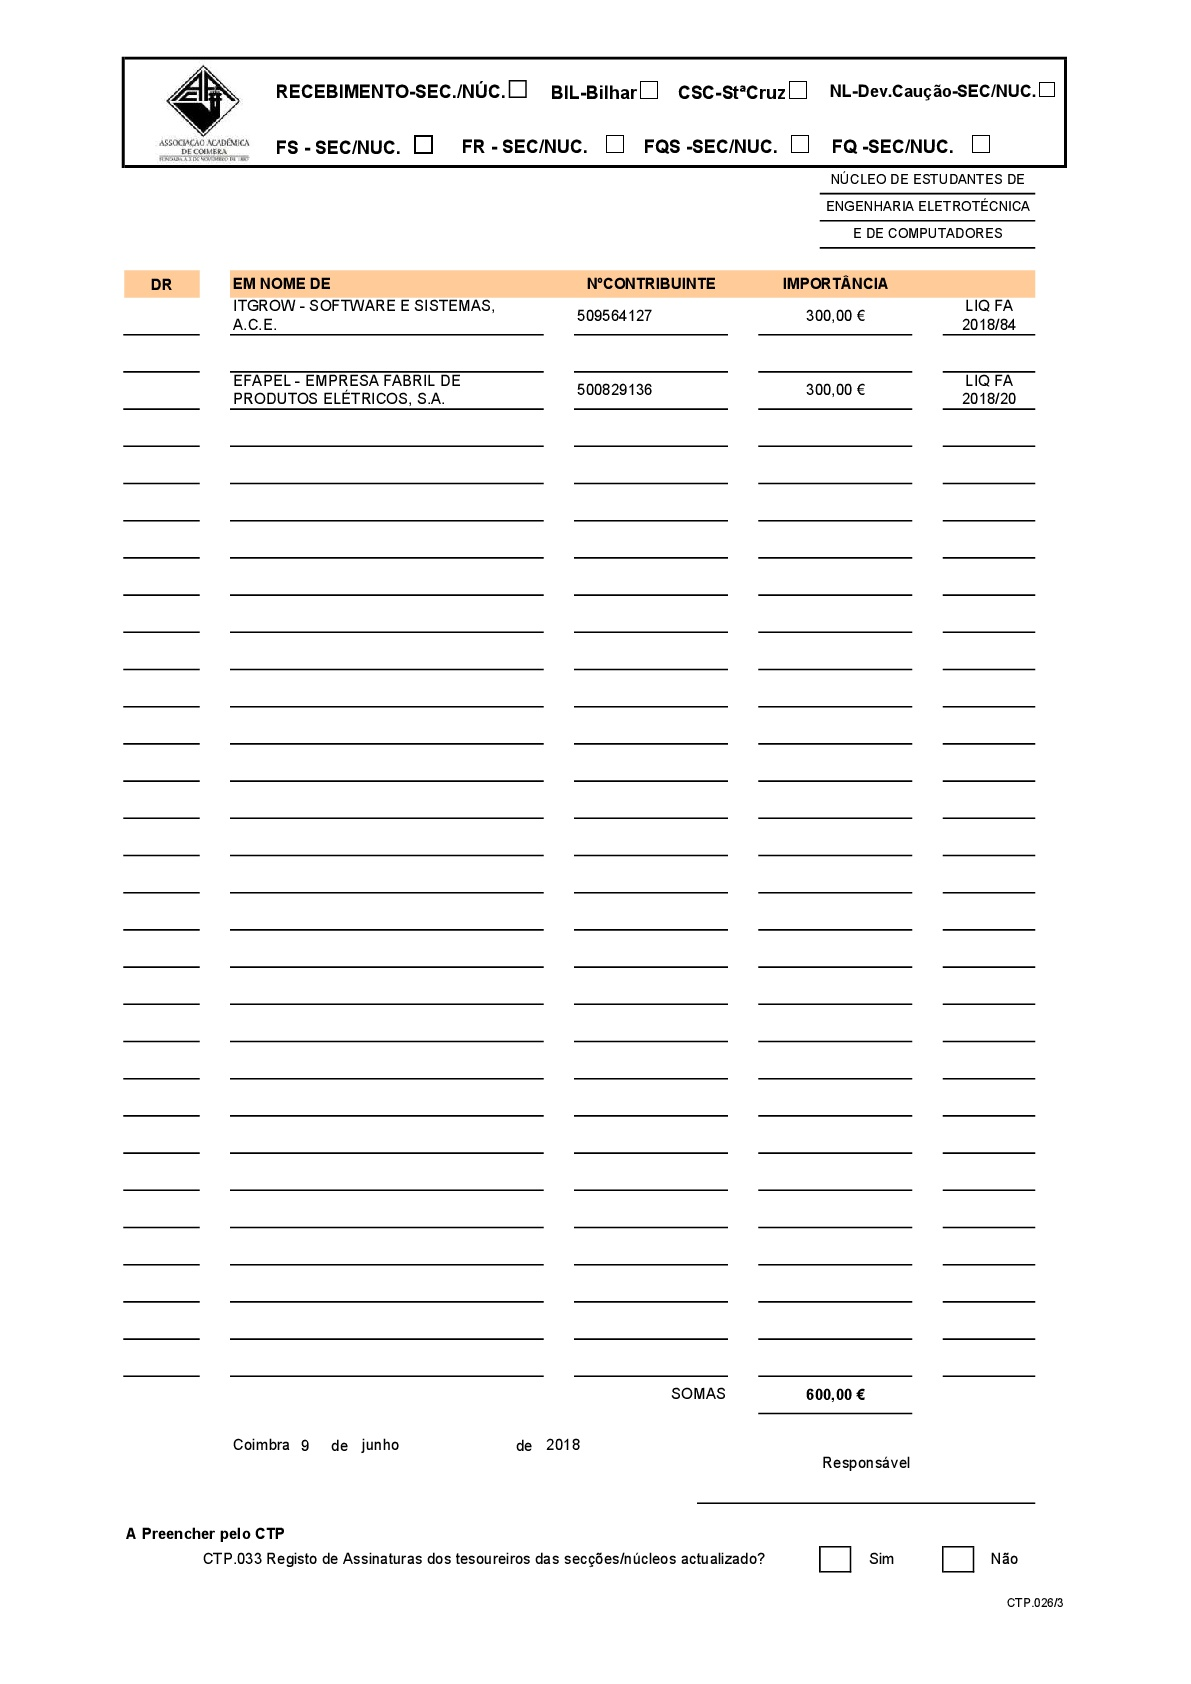
\includegraphics[width=\textwidth]{tesouraria/recibosFaturas}
        \caption{Pedido de recibos para faturas previamente emitidas.}
        \label{fig:Tesouraria-recibosFaturas}
    \end{subfigure}
    ~
    \begin{subfigure}[t]{0.3\textwidth}
        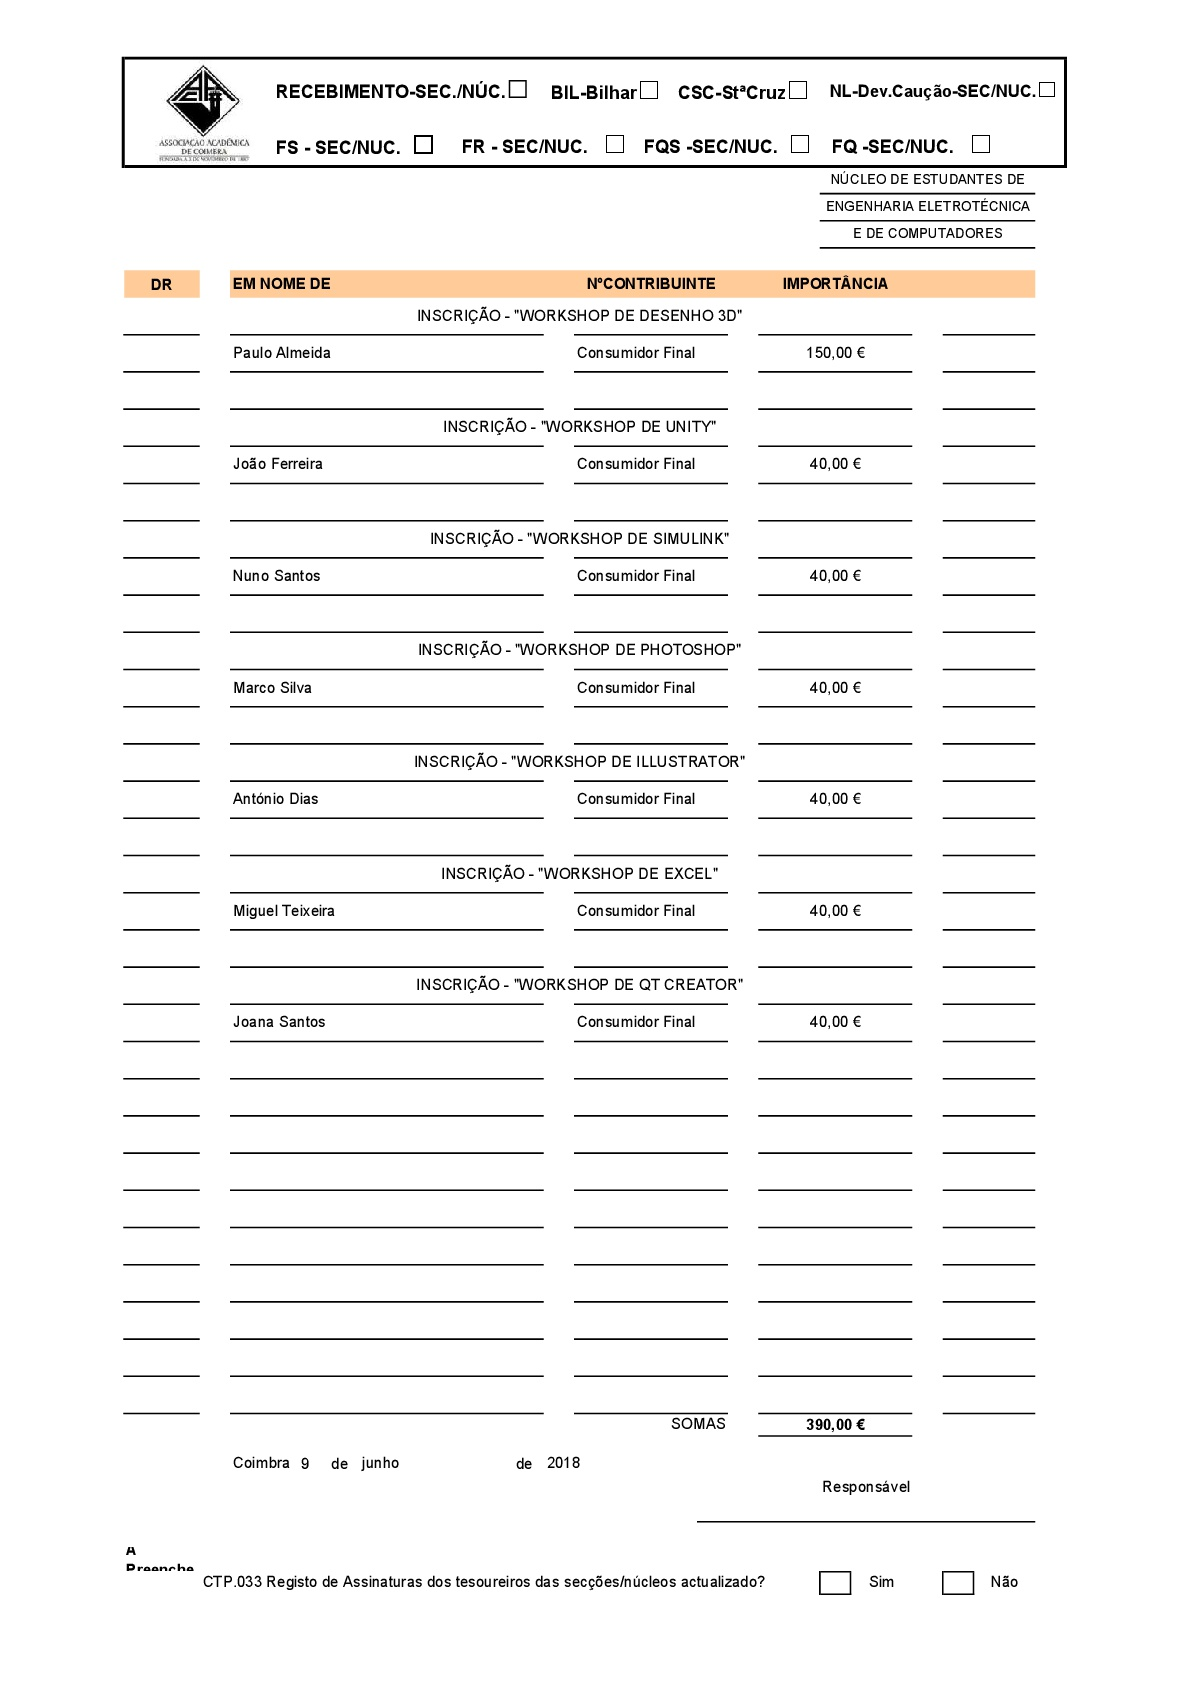
\includegraphics[width=\textwidth]{tesouraria/recibosInscricoes}
        \caption{Pedido de recibos para inscrições em atividades.}
        \label{fig:Tesouraria-recibosInscricoes}
    \end{subfigure}
    ~
    \begin{subfigure}[t]{0.3\textwidth}
        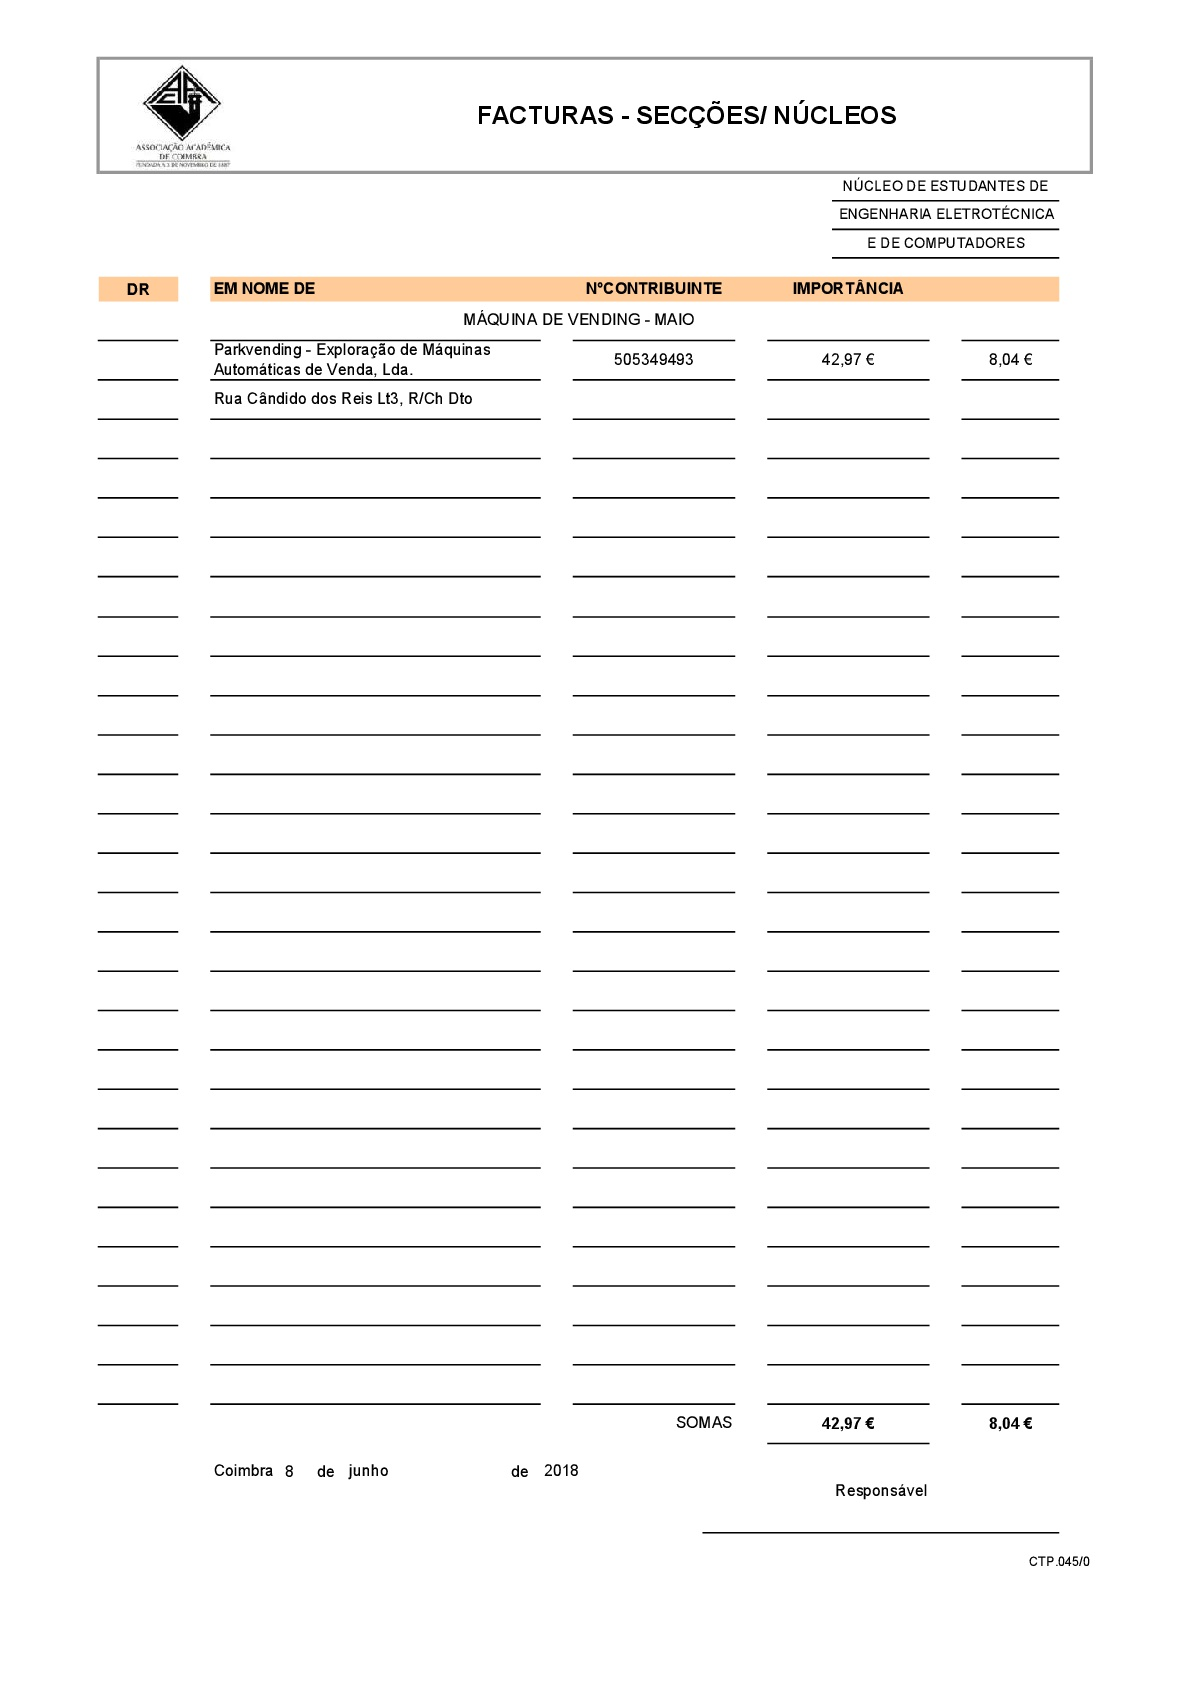
\includegraphics[width=\textwidth]{tesouraria/faturas}
        \caption{Pedido de faturas para pagamentos por realizar.}
        \label{fig:Tesouraria-faturas}
    \end{subfigure}
\end{figure}

\ifthenelse{\boolean{biblia}}
{ % TRUE
Exceto se pedido explicitamente pela pessoa, é recomendável agrupar os recibos das inscrições em atividades como "Consumidor Final"\space num recibo único para uma só pessoa, desde que o valor não ultrapasse os 199,99€, evitando a emissão de documentos inúteis. A partir do valor indicado, terão que ser emitidos múltiplos documentos até esse valor. No caso de pessoas que pedem o \acrshort{nif}, é obrigatório emitir individualmente cada recibo. Estes recibos pedidos explicitamente ou com o \acrshort{nif} devem ser entregues à pessoa, pelo que no decorrer do mandato, foram enviadas sempre digitalizações desses documentos por email, que poderão mais tarde levantar no Núcleo, caso o pretendam.
}
{ % FALSE
}

Quanto às faturas e recibos para empresas, cada empresa tem um método de trabalho distinto, pelo que para algumas empresas bastará enviar o documento digitalmente, enquanto que noutros casos é preciso enviar o mesmo por correio. Neste último caso, recomenda-se o aproveitamento dos modelos de carta e de envelopes já criados, adaptando apenas para o caso específico em questão. Recomenda-se ainda o envio da carta por correio registado, tendo assim sempre uma prova do envio da mesma, apesar dos custos associados a isso.

No caso de patrocínios em géneros, algumas empresas podem pedir um comprovativo desse apoio, como foi o caso do Pingo Doce este ano. Contudo, há que frisar que, no caso do Pingo Doce, das duas vezes que tal ocorreu, o mesmo homem pedia uma fatura dos apoios, o que implicaria pagar o \acrfull{iva}, contudo basta um documento certificativo emitido pelo \acrshort{ctp}, tal como será explicado caso seja feito esse pedido no gabinete do \acrshort{ctp}.

Por fim, há ainda o template de comprovativo de pagamento, que nunca chegou a ser utilizado este mandato. A utilização deste modelo chegou a ser pensado na altura do \acrshort{ene3}, pois houve devolução de inscrição a duas pessoas, contudo não se chegou a preenchê-lo dado que ainda não tinham sido emitidos os recibos dessas inscrições, pelo que a devolução anulou de imediato o valor recebido dessa pessoa.

Para que o preenchimento das informações dos documentos de Tesouraria, nomeadamente faturas, ficassem corretamente preenchidos e com os valores corretos, foi criado um modelo de faturação para simplificar o processo e permitir que, caso haja algum erro, a culpa seja tendencialmente da empresa. Este documento pede todo o tipo de informações necessárias, mas recomenda-se algumas alterações, nomeadamente na secção do montante do apoio para explicitar se o \acrshort{iva} está incluído, ou não, nesse valor.